\documentclass{beamer}
\newcommand\Fontvi{\fontsize{9}{11}\selectfont}
\newcommand\Fontcap{\fontsize{6}{8}\selectfont}
\newcommand\Fontot{\fontsize{7.5}{9}\selectfont}
%\bibliographystyle{./References/agu} 
\usepackage{amsmath}
\usepackage{amssymb}
\usepackage{graphicx}
\usepackage{url}
\usepackage{xfrac}
\usepackage{esvect}
\usepackage{varwidth} 
\usepackage{physics}
\usepackage{tensor}
\usepackage{microtype}

%%%%%%%%%%%%%%%%%%%%%%Multiple equations on the same line%%%%%%%%%%%%%%%%%%%%
\usepackage{multicol}
%%%%%%%%%%%%%%%%%%%%%%%%%%%%%%%%%%%%%%%%%
\newcommand{\driv}[2]{\frac{d #1}{d #2}}
\newcommand{\con}{\frac{8\pi}{3}G}
\newcommand{\brac}[1]{\left(#1\right)}
\newcommand{\bracc}[1]{\left[#1\right]}
%%%%%%%%%%%%%%%%%%%%%%%%%%%%%%%%%%%%%%%%%%                                        

\usepackage{multicol}
\usepackage{natbib}
\usepackage{amsmath}
%\usetheme{Madrid}
\usetheme{Marburg}
\setbeamertemplate{navigation symbols}{}
\setbeamertemplate{frame numbering}{fraction}
\usecolortheme[named=violet]{structure}

\setbeamercovered{transparent=5}
%\usebeamerfont{title}\insertsectionhead\par%

\makeatletter
\setbeamertemplate{sidebar canvas right}[vertical shading][top=black,bottom=violet]
\setbeamertemplate{footline}
{
\leavevmode%
\hbox{%
\begin{beamercolorbox}[wd=0.5\paperwidth, ht=2.25ex,dp=1ex, center]{author in head/foot}%
\usebeamerfont{author in head/foot}\insertauthor
\end{beamercolorbox}
\begin{beamercolorbox}[wd=0.5\paperwidth, ht=2.25ex,dp=1ex, right]{title in head/foot}%
\usebeamerfont{title in head/foot}
%\inserttitle \hspace*{0.5em}
\insertframenumber{}/\inserttotalframenumber\hspace*{2ex}
\end{beamercolorbox}}%
\vskip0pt%
}

\makeatother
\title{Solving the Friedman equation for a Dark Fluid equation of state.}
\subtitle{}
\author{Pieter vd Merwe}
\institute{North-West University Centre for Space Research}
\date{\today}

\begin{document}

\begin{frame}
\titlepage
%\begin{flushright}
%
\includegraphics[scale=0.3]{./Images/nwu_logo.jpg}
%\end{flushright}
%\begin{flushleft}
%\includegraphics[scale=0.4]{./Images/NASSP_logo.jpg}
%\end{flushleft}
\begin{figure}[ht]
    \begin{minipage}{0.45\linewidth}
        \centering
        \includegraphics[width=\textwidth]{./Images/NASSP_logo.jpg}
    \end{minipage}
    \begin{minipage}{0.45\linewidth}
        \centering
        
\includegraphics[width=\textwidth]{./Images/nwu_logo.jpg}
    \end{minipage}
\end{figure}
\end{frame}

\section{Introduction}
\begin{frame}
\frametitle{Introduction}
\begin{itemize}
\item \textbf{Cosmological principle:}\\
The universe is homogeneous and isotropic \citep{ITC}.
\item \textbf{General Relativity:}\\
Einstein`s field equations:
\begin{equation}\label{eq:GR}
\begin{split}
\tensor{G}{_{\mu\nu}}&=\frac{8\pi G}{c^{4}}\tensor{T}{_{\mu\nu}}+\Lambda\tensor{g}{_{\mu\nu}}\\
\end{split}
\end{equation}
\item \textbf{Hubble`s law:}
\begin{equation}\label{eq:Hubble}
\begin{split}
\nu&=H_{0}r.\\
\end{split}
\end{equation}
\item \textbf{Expanding universe:}
\begin{equation}\label{eq:scale}
\begin{split}
r(t) &= a(t)\chi.\\
\end{split}
\end{equation}

\end{itemize}
\end{frame}

\section{Friedmann equations}
\begin{frame}
\begin{itemize}
\frametitle{\insertsectionhead}

\item \textbf{Fluid equation:}
\begin{equation}\label{eq:6}
\begin{split}
\dot{\rho}+3H\left(1+\omega\right)\rho &= 0,\ \text{with } H=\frac{\dot{a}}{a}\\.
\end{split}
\end{equation}
\item \textbf{Friedmann equation:}
\begin{equation}
\begin{split}\label{eq:CurvFriedman}
\dot{a}^{2} &= \frac{8\pi G}{3c^{2}}\rho a^{2}-\kappa\frac{c^{2}}{\chi^{2}}\\
\end{split}
\end{equation}
\item \textbf{Raychaudhuri equation:}
\begin{equation}\label{eq:RayEq}
\begin{split}
\frac{\ddot{a}}{a} &= -\frac{4\pi}{3}G\left(\rho +3P\right)\\
\end{split}
\end{equation}

\end{itemize}
\end{frame}

\section{Concordance model ($\Lambda$CDM-model)}
\begin{frame}
\begin{itemize}
\frametitle{\insertsectionhead}

\item \textbf{Dark Matter.}
\item \textbf{Accelerated expansion:}\\
Observations of the luminosities of type Ia supernovae suggest that the universe is undergoing an accelerated expansion \citep{NPSNe, RMCGAU}, which suggests the existence of a Dark energy element.
\item \textbf{Assume a perfect fluid equation of state:}
\begin{equation}\label{eq:PFEoS}
\begin{split}
P &= \omega\rho         \\
\end{split}
\end{equation}
\item \textbf{3 Different epochs:}
\begin{itemize}
\item[$-$] Radiation ($\omega=\frac{1}{3}$): $\rho=C_{rad}a^{-4}$ \\
\item[$-$] Matter ($\omega=0$): $\rho=C_{dust}a^{-3}$ \\
\item[$-$] Dark Energy ($\omega=-1$): $\rho=C_{DE}$\\
\end{itemize}

\end{itemize}
\end{frame}

\section{Chaplygin gas}
\begin{frame}
\begin{itemize}
\frametitle{\insertsectionhead}
\item Different Chaplygin gas equations of state \citep{kahya2015universe}:
\begin{itemize}
\item[$-$] Original Chaplygin gas (OCG):
\begin{equation}\label{eq:OCG}
\begin{split}
P &= -\frac{A_{1}}{\rho}.         \\
\end{split}
\end{equation}
\item[$-$] Generalised Chaplygin gas (GCG):
\begin{equation}\label{eq:GCG}
\begin{split}
P &= -\frac{A_{1}}{\rho^{\alpha}},\ \ \ \ \alpha>-1.         \\
\end{split}
\end{equation}
\item[$-$] Modified Chaplygin gas (MCG):
\begin{equation}\label{eq:MCG}
\begin{split}
P &=A_{2}\rho -\frac{A_{1}}{\rho^{\alpha}},\ \ \ \ \alpha>-1.        \\
\end{split}
\end{equation}
\end{itemize}
\end{itemize}
\end{frame}


\subsection{Solution to the fluid equation}
\begin{frame}
\begin{itemize}
\fontsize{8pt}{7.2}\selectfont
\frametitle{\insertsectionhead}
\framesubtitle{\insertsubsectionhead}

\item \textbf{Solving the Fluid equation for a MCG equation of state:}
\begin{equation}\label{eq:FMCGZ}
\begin{split}
\rho  &= \bracc{\frac{C_{2}\brac{1+z}^{3\brac{\alpha+1}\brac{1+A_{2}}}+A_{1}}{1+A_{2}}}^{\frac{1}{1+\alpha}},         \\
\end{split}
\end{equation}

\end{itemize}
\begin{figure}[h]
\centering
\includegraphics[scale=0.45]{Images/ch_rho.jpg}
\caption{Here we have taken $A_{1}=50$, $A_{2}=C_{2}=1$ and $\alpha=1$. }
\label{fig:ChRho}
\end{figure}
\end{frame}

\subsection{Solving the Friedmann equation for the MCG equation of state}
\begin{frame}
\begin{itemize}
\frametitle{\insertsectionhead}
\framesubtitle{\insertsubsectionhead}
\fontsize{7pt}{7.2}\selectfont
\item Assuming a $\kappa=0$, we have:
\fontsize{6pt}{7.2}\selectfont
\begin{equation}\label{eq:FmEqMCGSol}
\begin{split}
\brac{t-t_{0}}&=\frac{2}{3A^{\frac{1}{2}}B_{2}^{\frac{1}{2\beta}}B_{1}}\brac{\frac{B_{3}}{B_{2}}a^{-3B_{1}\beta}+1}^{-\frac{1}{2\beta}}\\
+\frac{1}{2\beta+1}&\brac{\frac{B_{3}}{B_{2}}a^{-3B_{1}\beta}+1}^{-1-\frac{1}{2\beta}}\ _{2}F_{1}\brac{1,1+\frac{1}{2\beta};2+\frac{1}{2\beta};\brac{\frac{B_{3}}{B_{2}}a^{-3B_{1}\beta}+1}^{-1}},\\
\end{split}
\end{equation}
\end{itemize}
\begin{figure}[H]
\centering
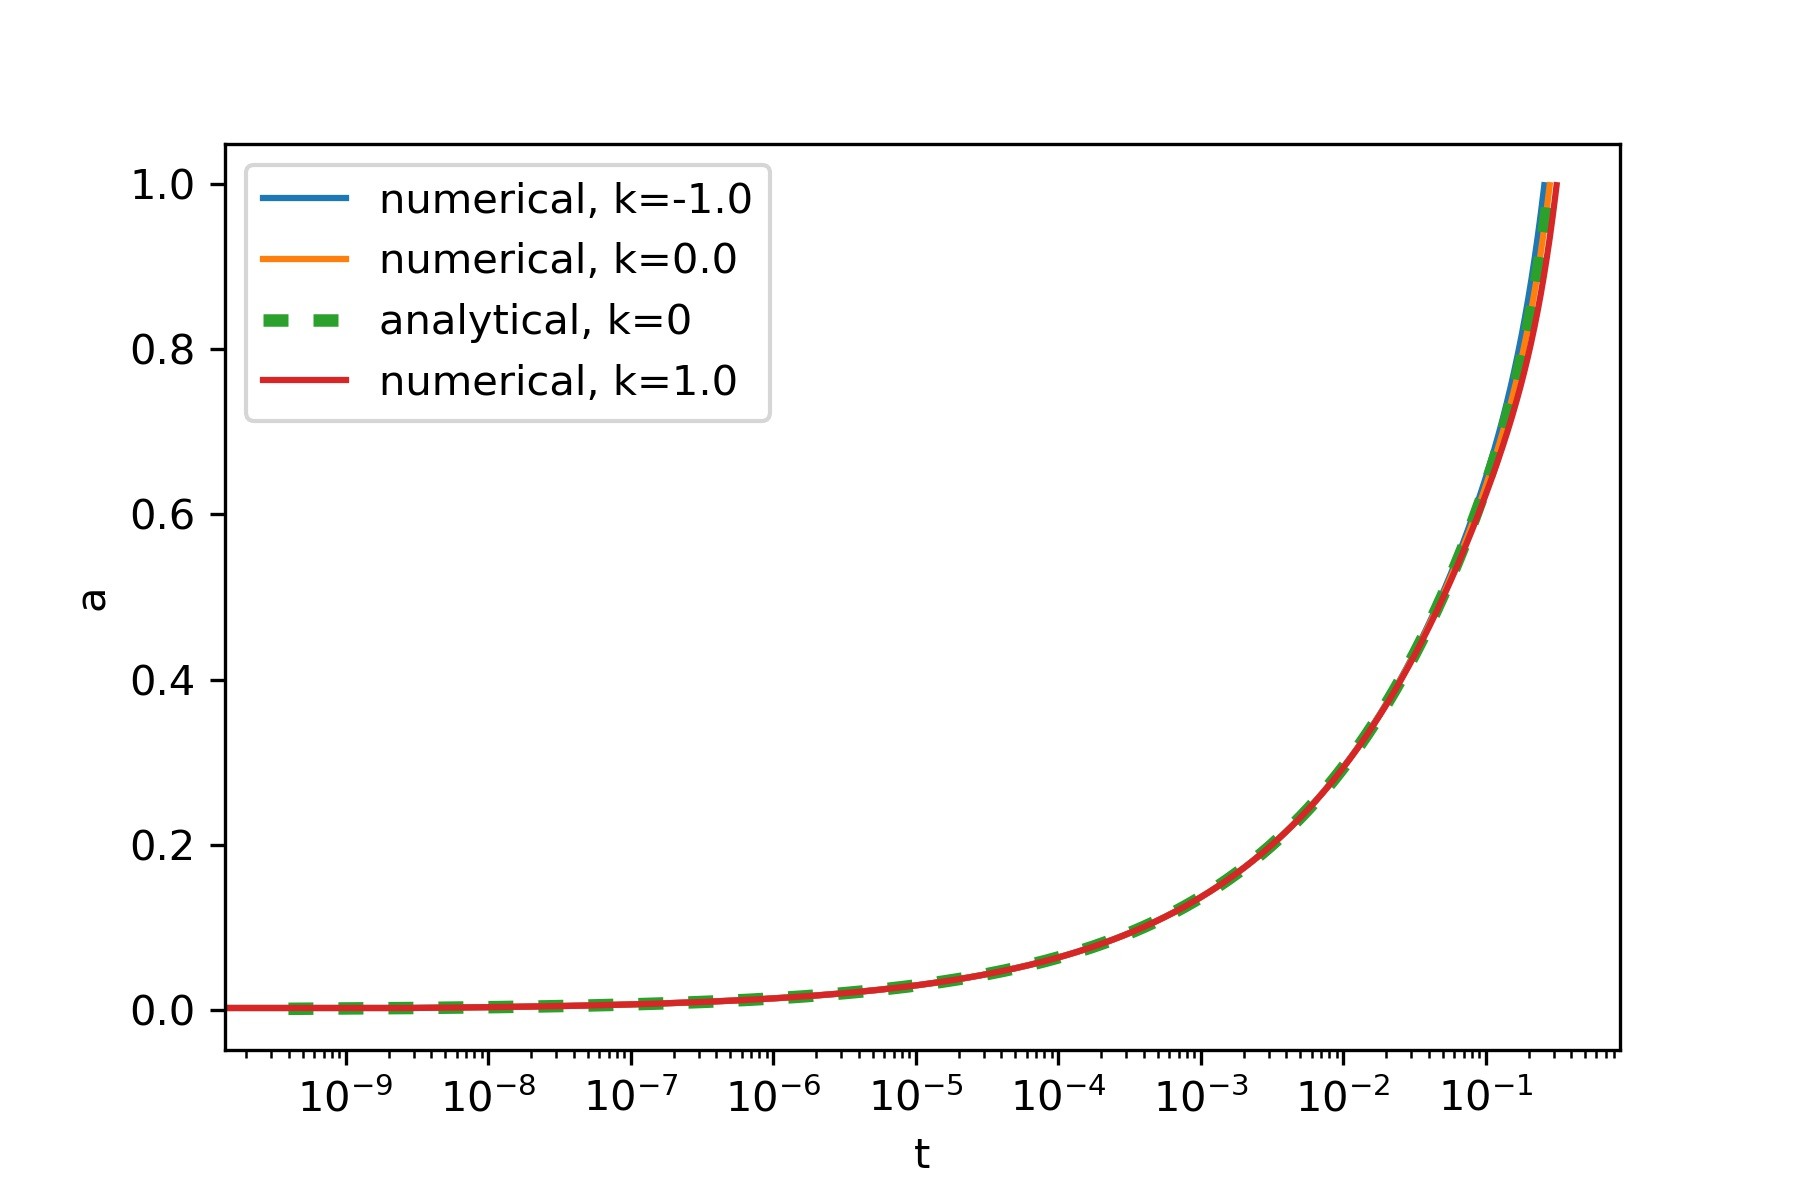
\includegraphics[scale=0.45]{Images/a_ch.jpg}
%\caption{Here equation (\ref{eq:NumSolMCG}) has been integrated numerically for $a'=0$ to $a'=1$ in incremental steps using the Gauss quadrature method. For this we have set $\frac{8\pi G}{3c^{2}}=\frac{c^{2}}{\chi^{2}}=1$ in order to investigate the behaviour of the model without looking at the physical constraints, and taken all of the free parameters to be the same as in the previous case. }
\label{fig:ChScale}
\end{figure}
\end{frame}

\subsection{Hubble parameter for MCG case}
\begin{frame}
\frametitle{\insertsectionhead}
\framesubtitle{\insertsubsectionhead}
\fontsize{8pt}{7.2}\selectfont
\begin{itemize}
\item Dimensionless Hubble parameter $h$
\begin{equation}\label{eq:zChDimHubbleParm}
\begin{split}
h(z) &= \frac{1}{H_{0}}\bracc{A\brac{B_{3}\brac{1+z}^{3\brac{\beta}\brac{B_{1}}}+B_{2}}^{\frac{1}{\beta}} -\kappa F\brac{1+z}^{2}}^{\frac{1}{2}}.\\
\end{split}
\end{equation}
\item Fractional energy density $\Omega$
\begin{equation}\label{eq:ChFracEnDen}
\begin{split}
\Omega_{Chap}(z) &\equiv \frac{A}{H_{0}^{2}}\brac{B_{3}\brac{1+z}^{3\brac{\beta}\brac{B_{1}}}+B_{2}}^{\frac{1}{\beta}} \\
\Omega_{\kappa}(z)&\equiv -\frac{\kappa F}{H_{0}^{2}}\brac{1+z}^{2}.\\
\end{split}
\end{equation}
\end{itemize}

\begin{figure}[ht]
    \begin{minipage}{0.49\linewidth}
        \centering
        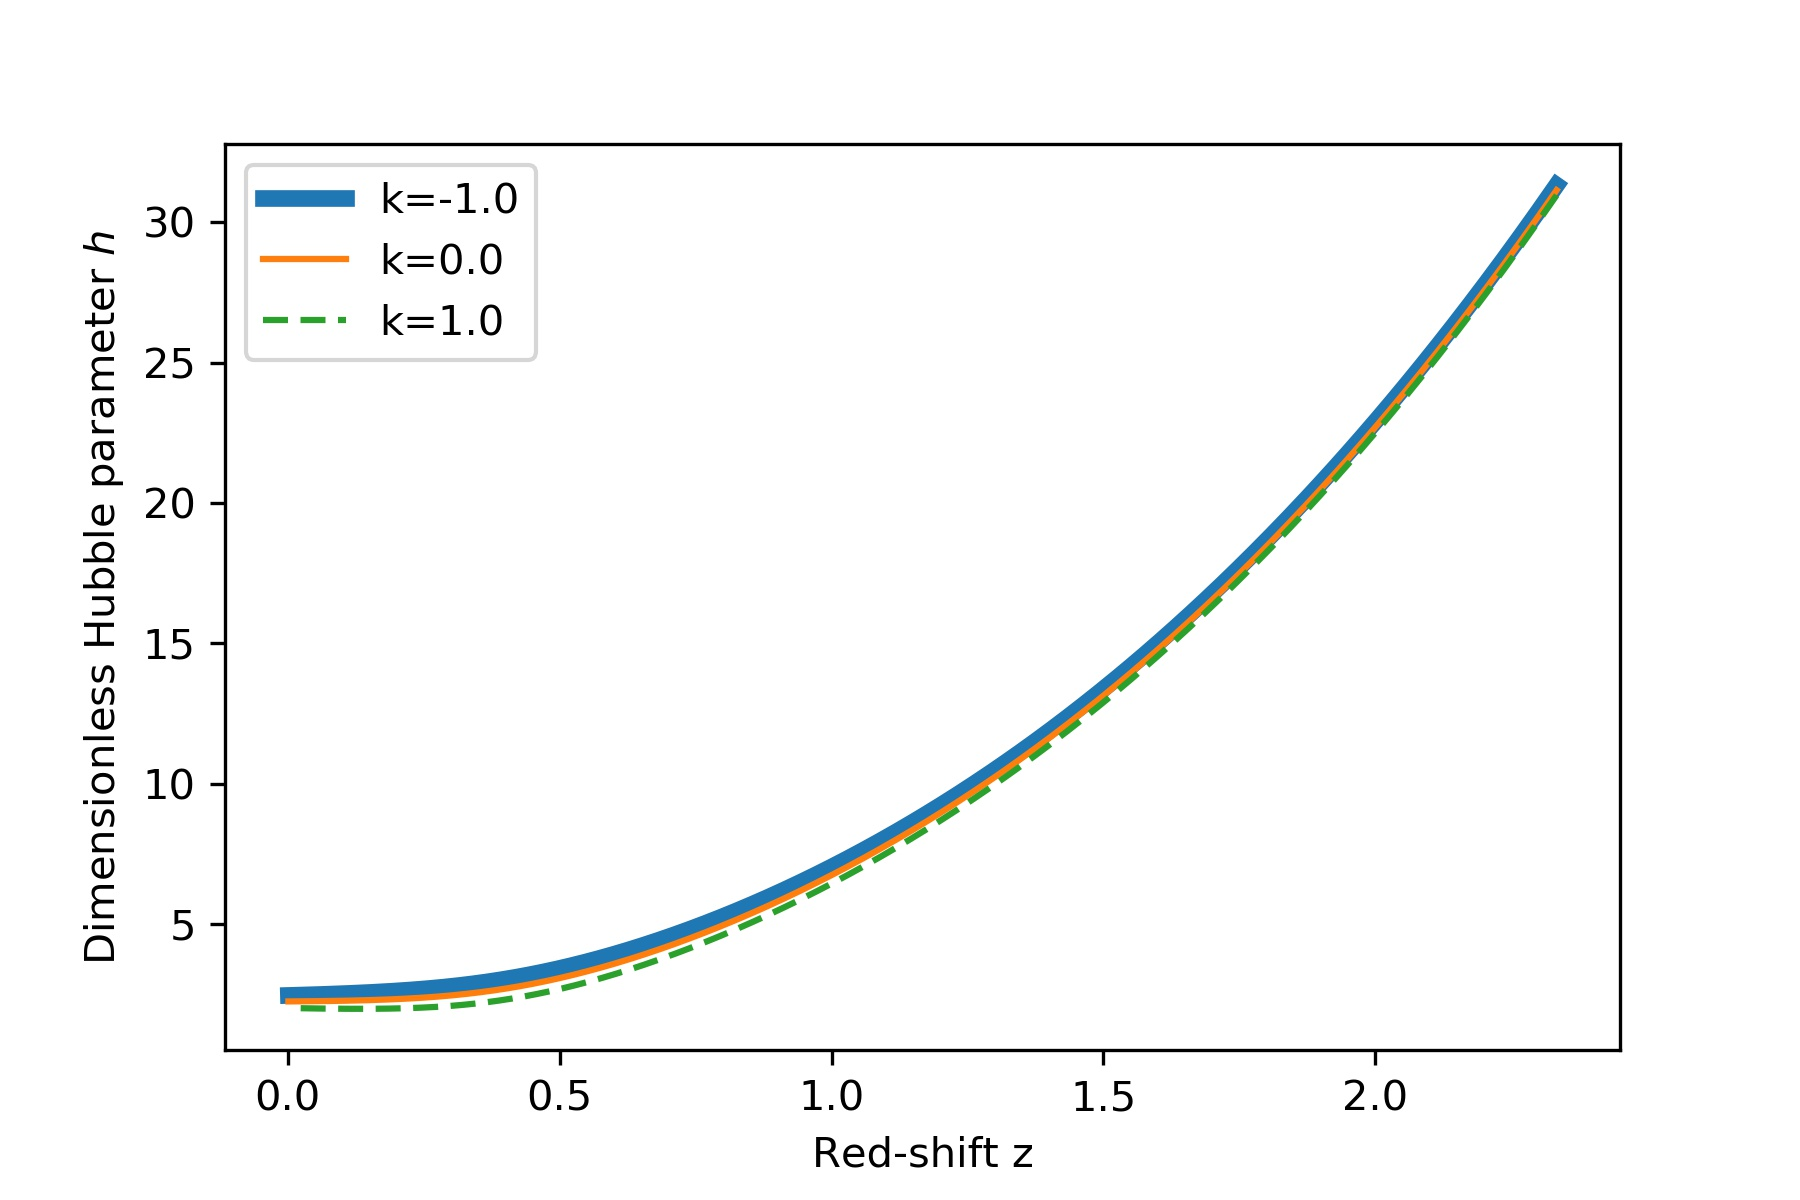
\includegraphics[width=\textwidth]{./Images/ch_H.jpg}
		%\caption{Here the Parameters have, again, been taken as in the previous cases and 			we have also set $H_{0}=1$.}
		\label{fig:ChH}
    \end{minipage}
    \begin{minipage}{0.49\linewidth}
        \centering
        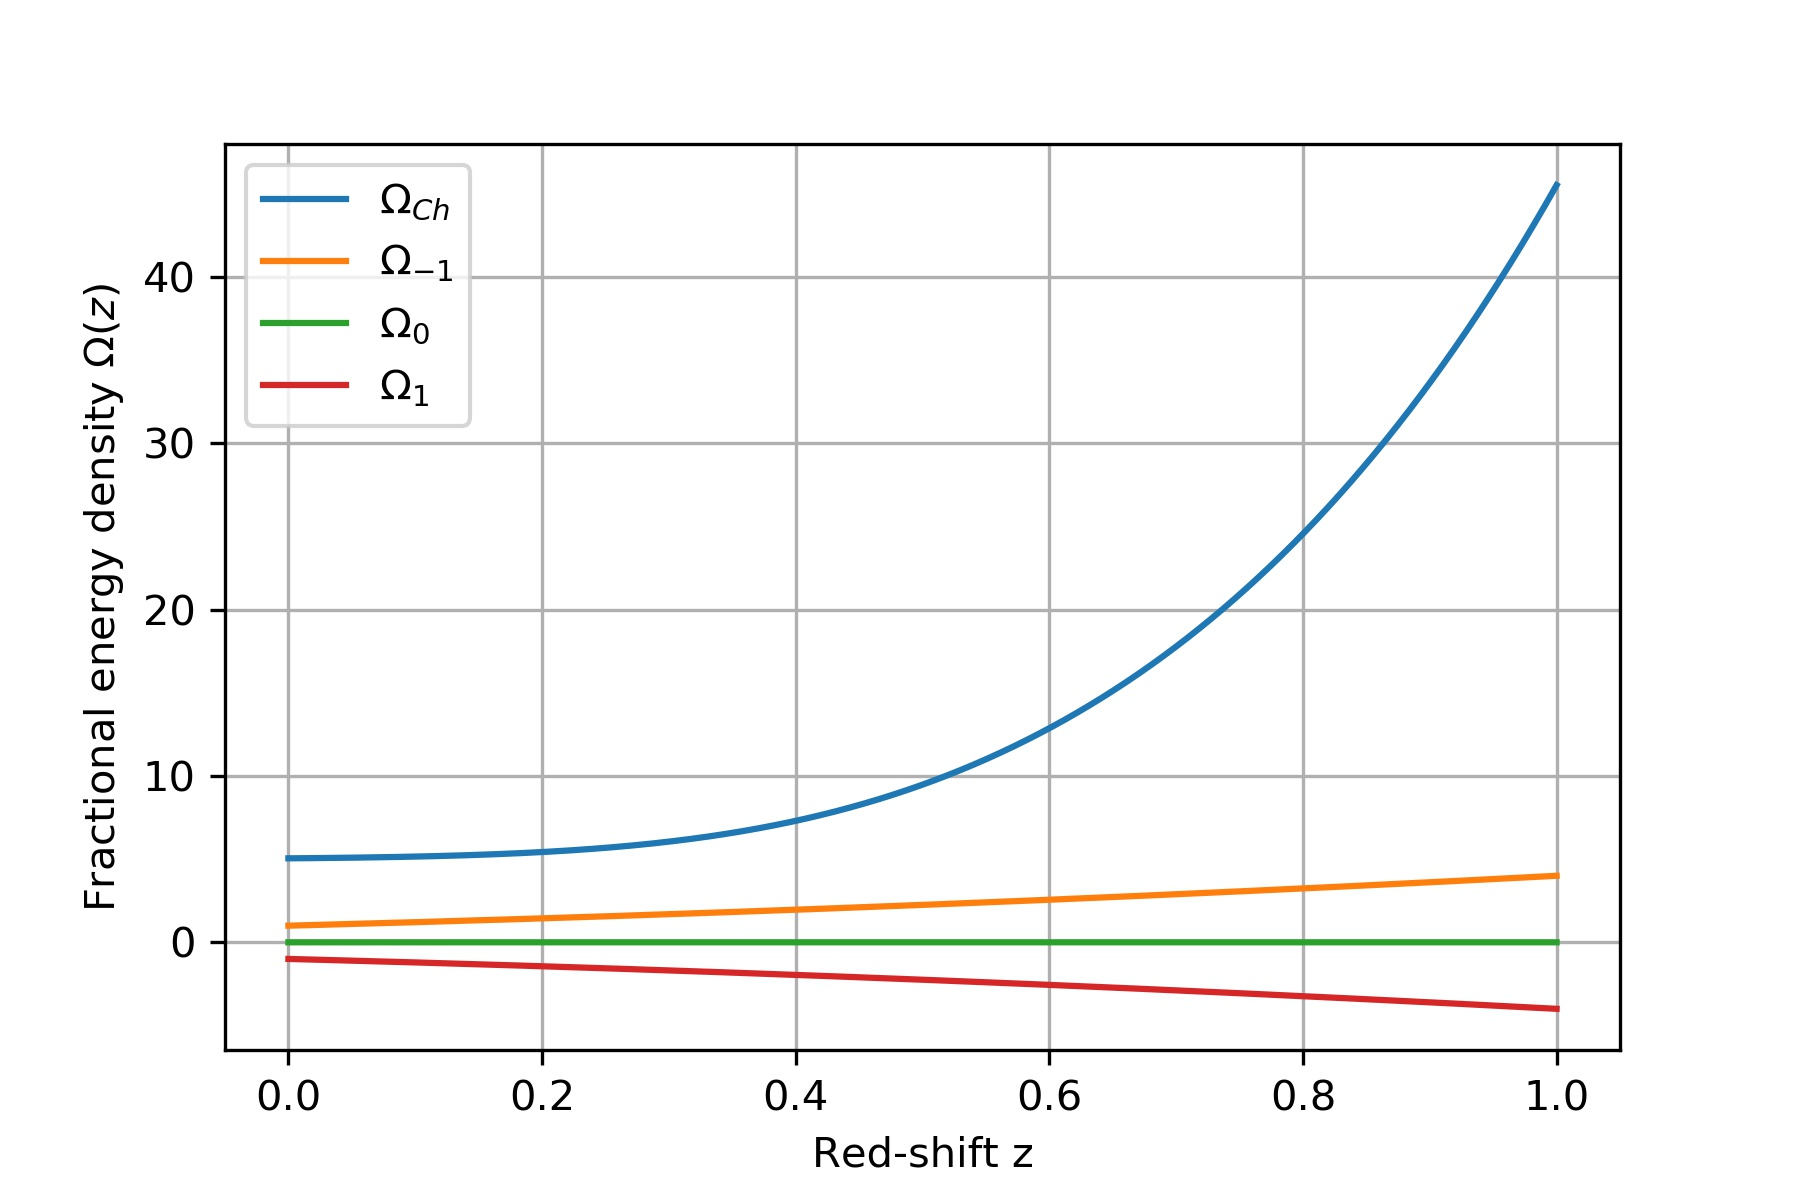
\includegraphics[width=\textwidth]{./Images/ch_Om.jpg}
		%\caption{Taking the various parameters as in the previous cases, the figure shows 			the fractional energy density of the Chaplygin gas fluid as well as for the 				different curvature cases.It is important to point out here that the fractional 			energy density of the different curvatures are non-linear, but increases much 				slower than the Chaplygin gas fractional energy density for the chosen parameters.}
		\label{fig:ChFracEnDen}
    \end{minipage}
\end{figure}

\end{frame}

\subsection{Acceleration of a for MCG case}
\begin{frame}
\frametitle{\insertsectionhead}
\framesubtitle{\insertsubsectionhead}
\fontsize{8pt}{7.2}\selectfont
\begin{itemize}
\item Acceleration of a:
\fontsize{6pt}{7.2}\selectfont
\begin{equation}\label{eq:ChRaych}
\begin{split}
\frac{\ddot{a}}{a} &= -\frac{A}{2}\brac{\brac{3B_{1}-2}\brac{B_{3}a^{-3B_{1}\beta}+B_{2}}^{\frac{1}{\beta}}-3B_{1}B_{2}\brac{B_{3}a^{-3\beta B_{1}}+B_{2}}^{\frac{1-\beta}{\beta}}},\\
\end{split}
\end{equation}
\fontsize{8pt}{7.2}\selectfont
\item Deceleration parameter $q\equiv-\frac{\ddot{a}a}{\dot{a}^{2}}$
\fontsize{6pt}{7.2}\selectfont
\begin{equation}\label{eq:ChModDecelZ}
\begin{split}
q &= \frac{\frac{A}{2}\brac{\brac{3B_{1}-2}\brac{B_{3}\brac{1+z}^{3B_{1}\beta}+B_{2}}^{\frac{1}{\beta}}-3B_{1}B_{2}\brac{B_{3}\brac{1+z}^{3\beta B_{1}}+B_{2}}^{\frac{1-\beta}{\beta}}}}{A\brac{B_{3}\brac{1+z}^{3\brac{\beta}\brac{B_{1}}}+B_{2}}^{\frac{1}{\beta}} -\kappa F\brac{1+z}^{2}}.
\end{split}
\end{equation}
\end{itemize}

\begin{figure}[ht]
    \begin{minipage}{0.49\linewidth}
        \centering
        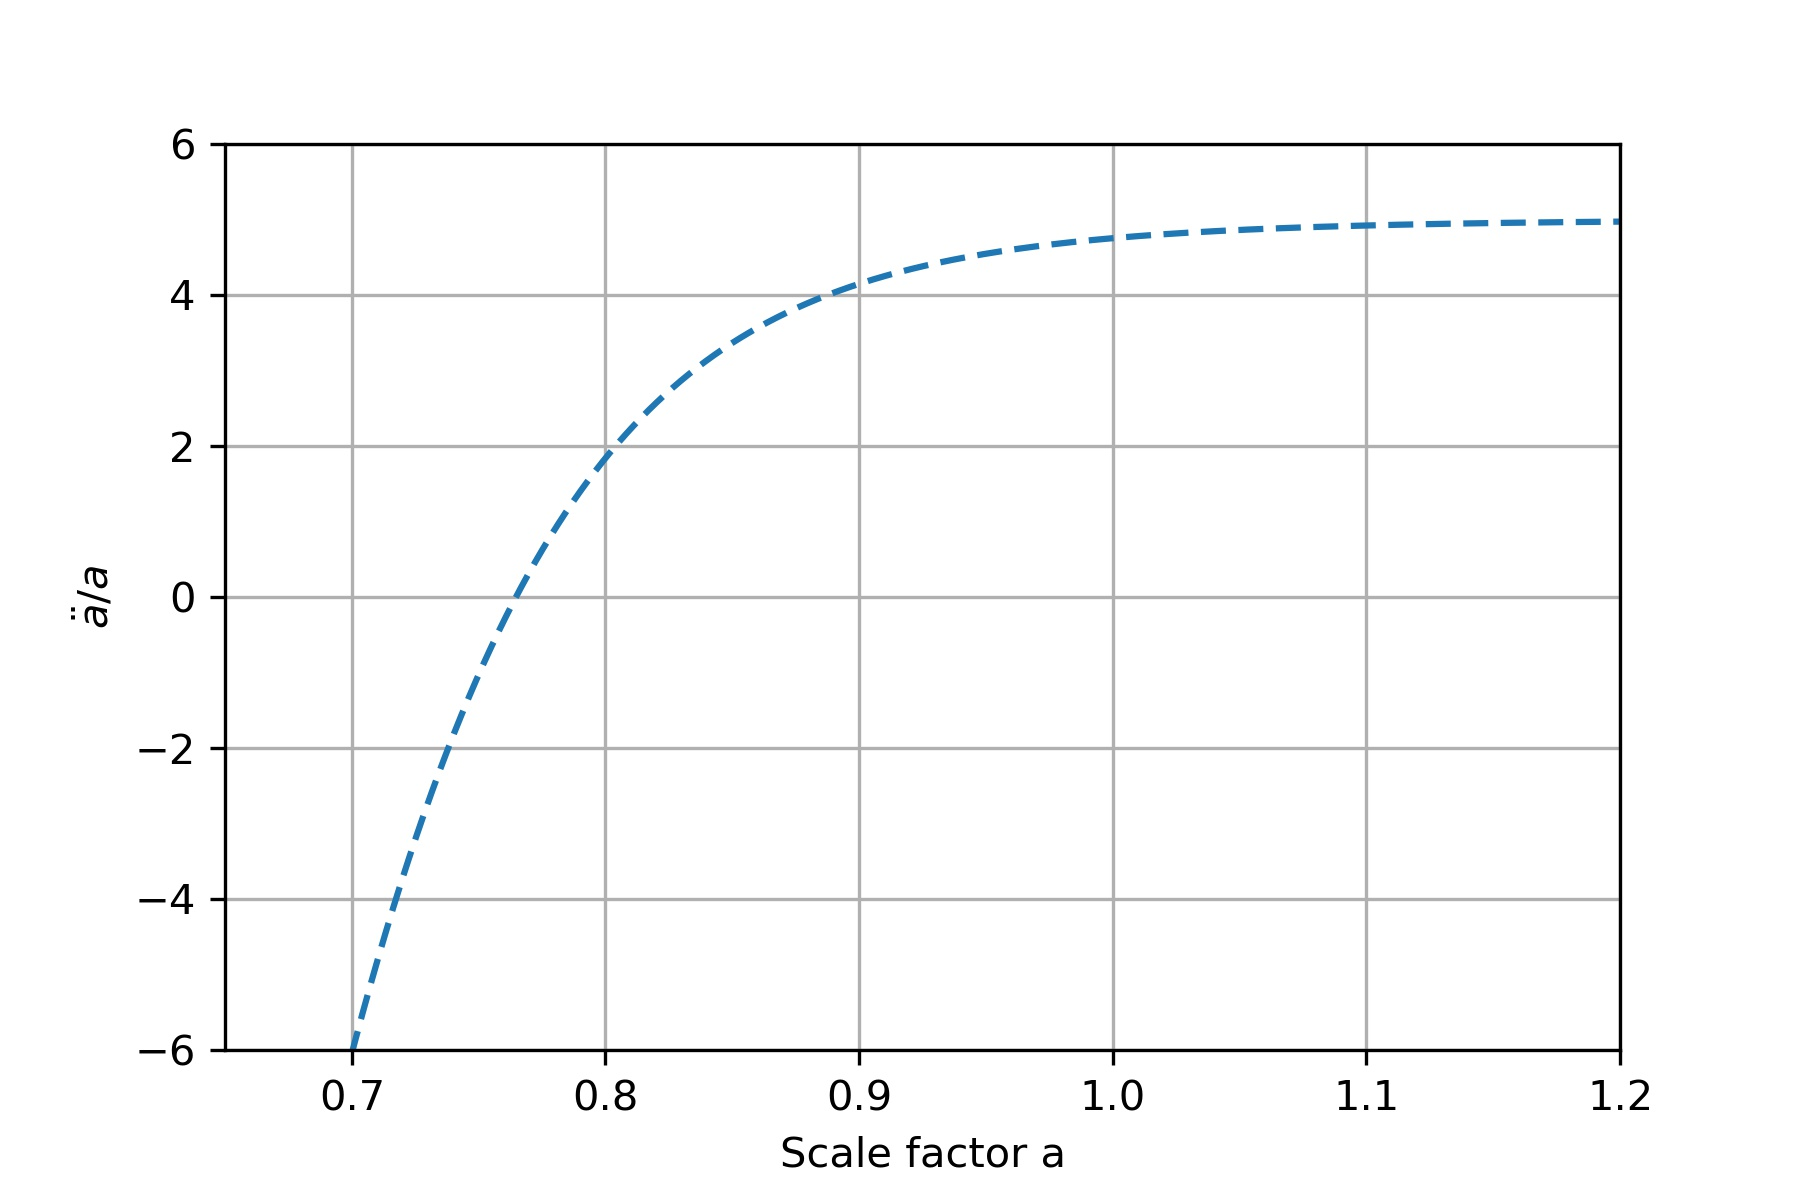
\includegraphics[width=\textwidth]{./Images/ch_ddota.jpg}
		\label{fig:ch_ddot}
    \end{minipage}
    \begin{minipage}{0.49\linewidth}
        \centering
        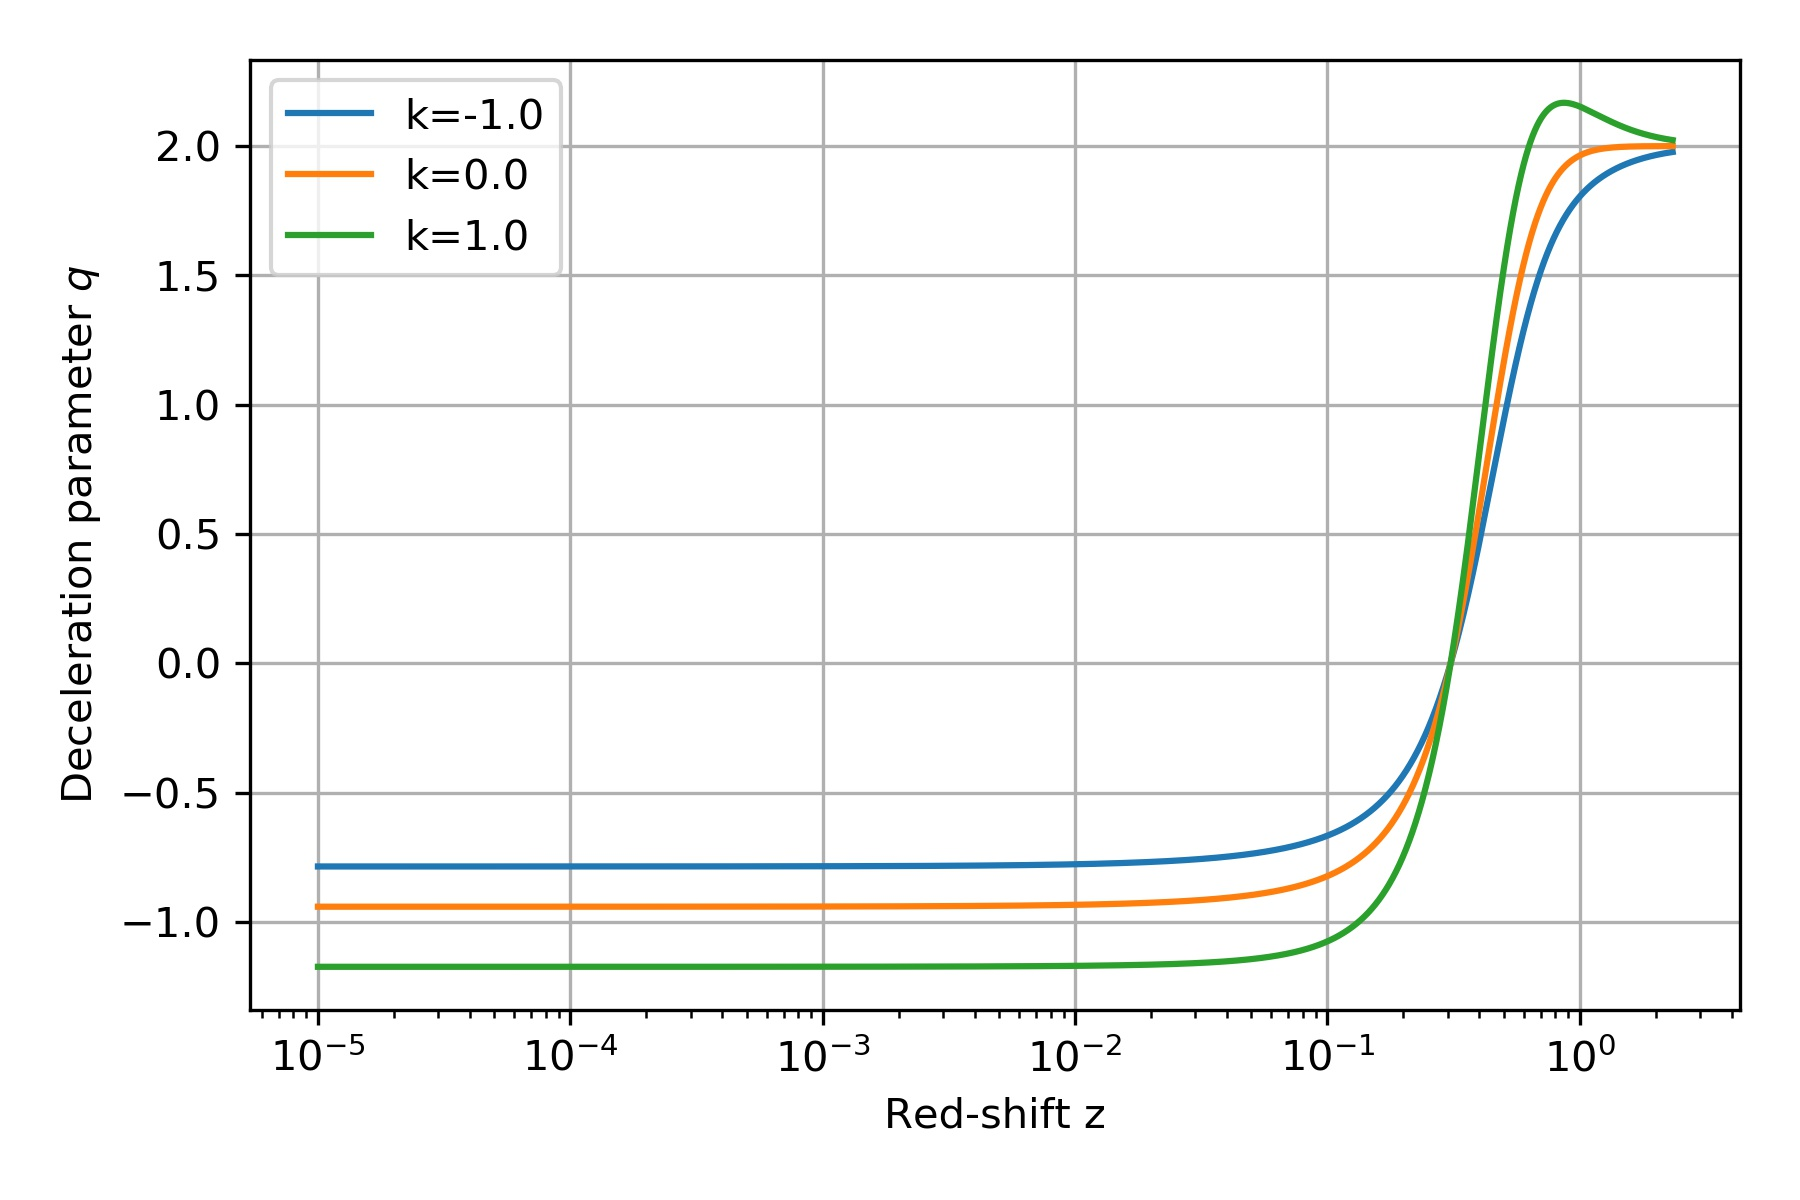
\includegraphics[width=\textwidth]{./Images/ch_q.jpg}
		\label{fig:Chq}
    \end{minipage}
\end{figure}
\end{frame}

\section{Pressure-Parametrized Unified Dark Fluid (PPUDF)}
\subsection{Solution to the fluid equation}
{
\setbeamerfont{frametitle}{size=\small}
\begin{frame}
\begin{itemize}
\frametitle{\insertsectionhead}
\fontsize{7pt}{7.2}\selectfont
\item \textbf{The PPUDF equation of state \citep{wang2017new}:}
\begin{equation}\label{eq:UDFEoS}
\begin{split}
P &= P_{a}+P_{b}\brac{z+\frac{z}{1+z}},         \\
\end{split}
\end{equation}
\item \textbf{Solving the Fluid equation for a PPUDF equation of state:}
\begin{equation}\label{eq:UDFFluidSolZ}
\begin{split}
\rho&= -P_{a}+\frac{3}{4}P_{b}\bracc{\brac{1+z}^{-1}-2\brac{1+z}}+C\brac{1+z}^{3}, \\
\end{split}
\end{equation}

\end{itemize}
\begin{figure}[h]
\centering
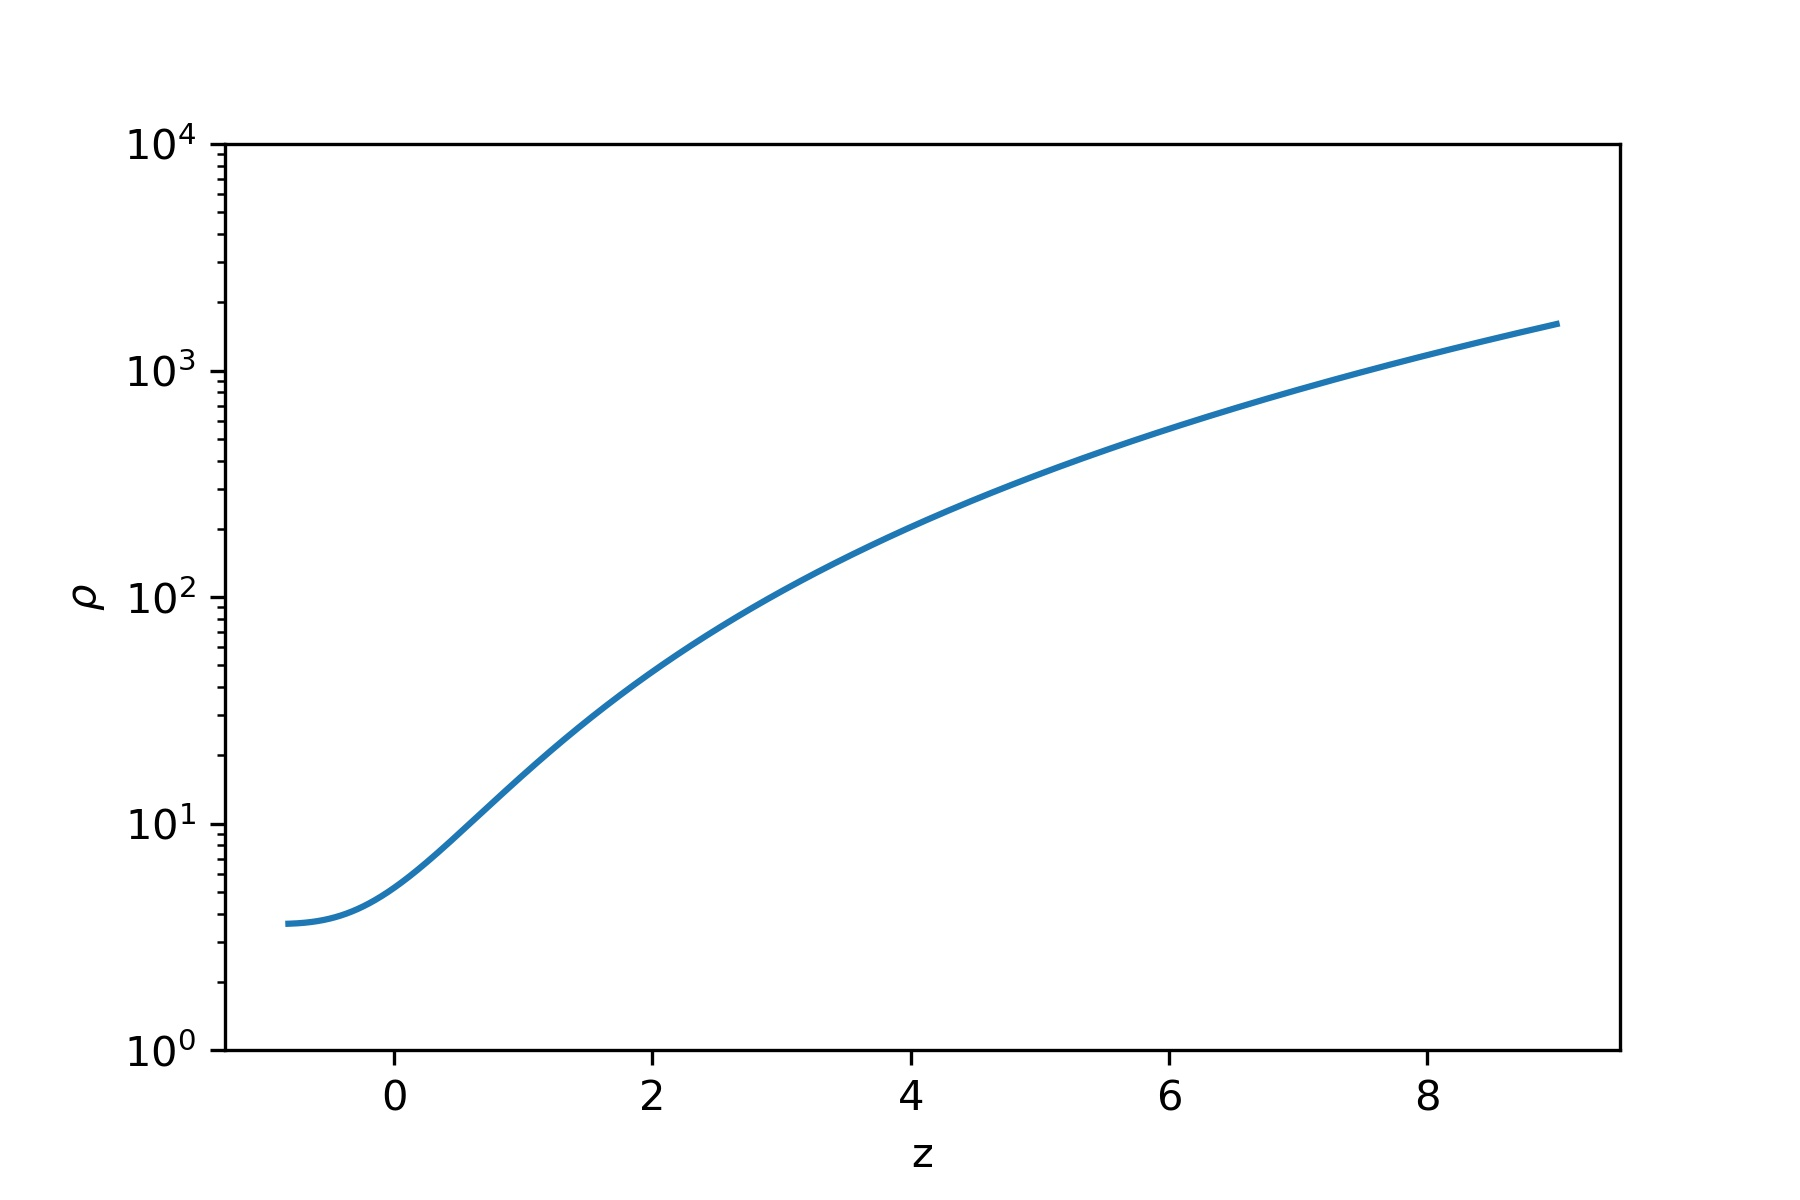
\includegraphics[scale=0.45]{Images/UDF_rho.jpg}
\label{fig:UDFRho}
\end{figure}
\end{frame}

\subsection{Hubble parameter for PPUDF case}
\begin{frame}
\frametitle{\insertsectionhead}
\framesubtitle{\insertsubsectionhead}
\fontsize{8pt}{7.2}\selectfont
\begin{itemize}
\item Dimensionless Hubble parameter $h$
\fontsize{6pt}{7.2}\selectfont
\begin{equation}\label{eq:UDFDimh}
\begin{split}
h &= \frac{1}{H_{0}}\bracc{A\brac{-P_{a}+\frac{3}{4}P_{b}\bracc{\brac{1+z}^{-1}-2\brac{1+z}}+C\brac{1+z}^{3}} -\kappa F \brac{1+z}^{2}}^{\frac{1}{2}}.\\
\end{split}
\end{equation}
\fontsize{8pt}{7.2}\selectfont
\item Fractional energy density $\Omega$
\fontsize{6pt}{7.2}\selectfont
\begin{equation}\label{eq:UDFOmega}
\begin{split}
\Omega_{PPUDF}(z) &\equiv \frac{A}{H_{0}^{2}}\brac{-P_{a}+\frac{3}{4}P_{b}\bracc{\brac{1+z}^{-1}-2\brac{1+z}}+C\brac{1+z}^{3}}      \\
\Omega_{\kappa}(z)&\equiv -\frac{\kappa F}{H_{0}^{2}}\brac{1+z}^{2}.\\
\end{split}
\end{equation}
\end{itemize}

\begin{figure}[ht]
    \begin{minipage}{0.49\linewidth}
        \centering
        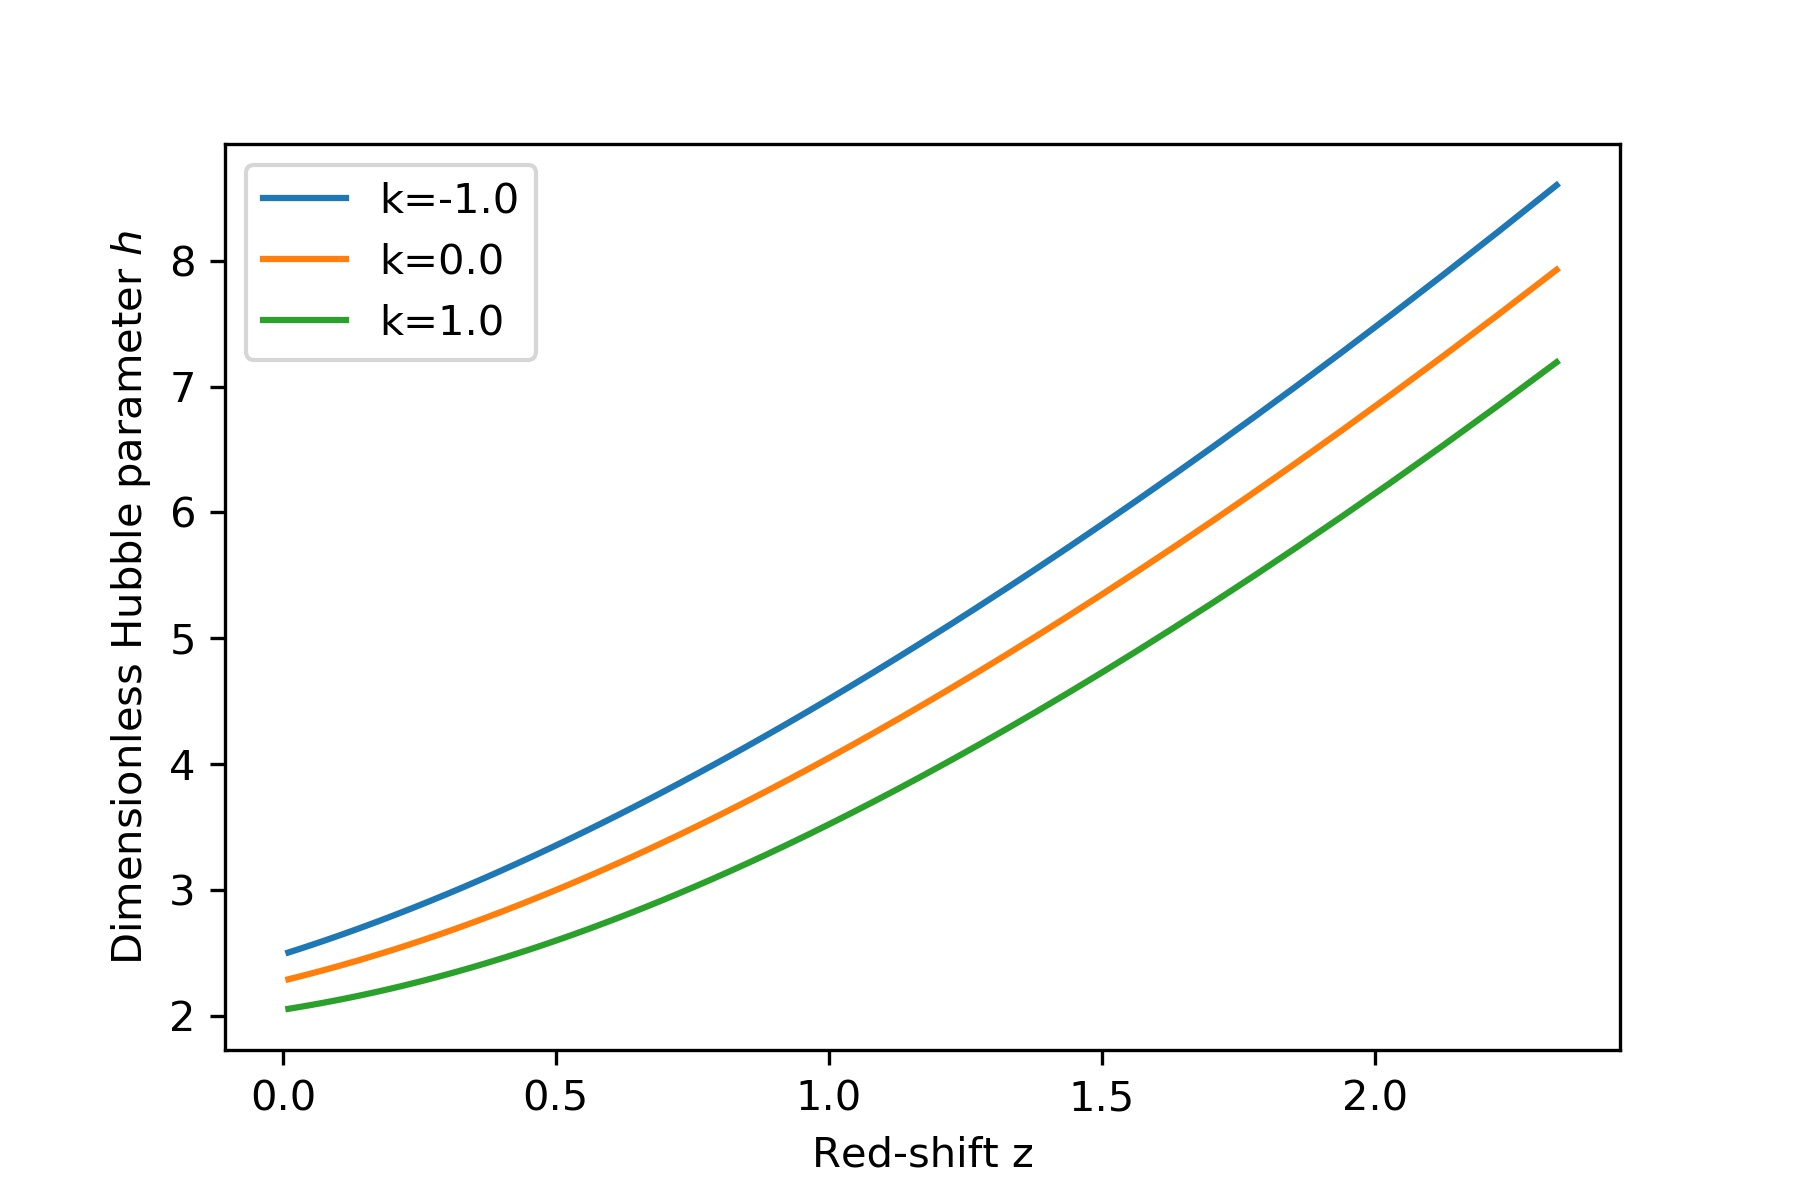
\includegraphics[width=\textwidth]{./Images/UDF_H.jpg}
		%\caption{Here the Parameters have, again, been taken as in the previous cases and 			we have also set $H_{0}=1$.}
		\label{fig:UDFH}
    \end{minipage}
    \begin{minipage}{0.49\linewidth}
        \centering
        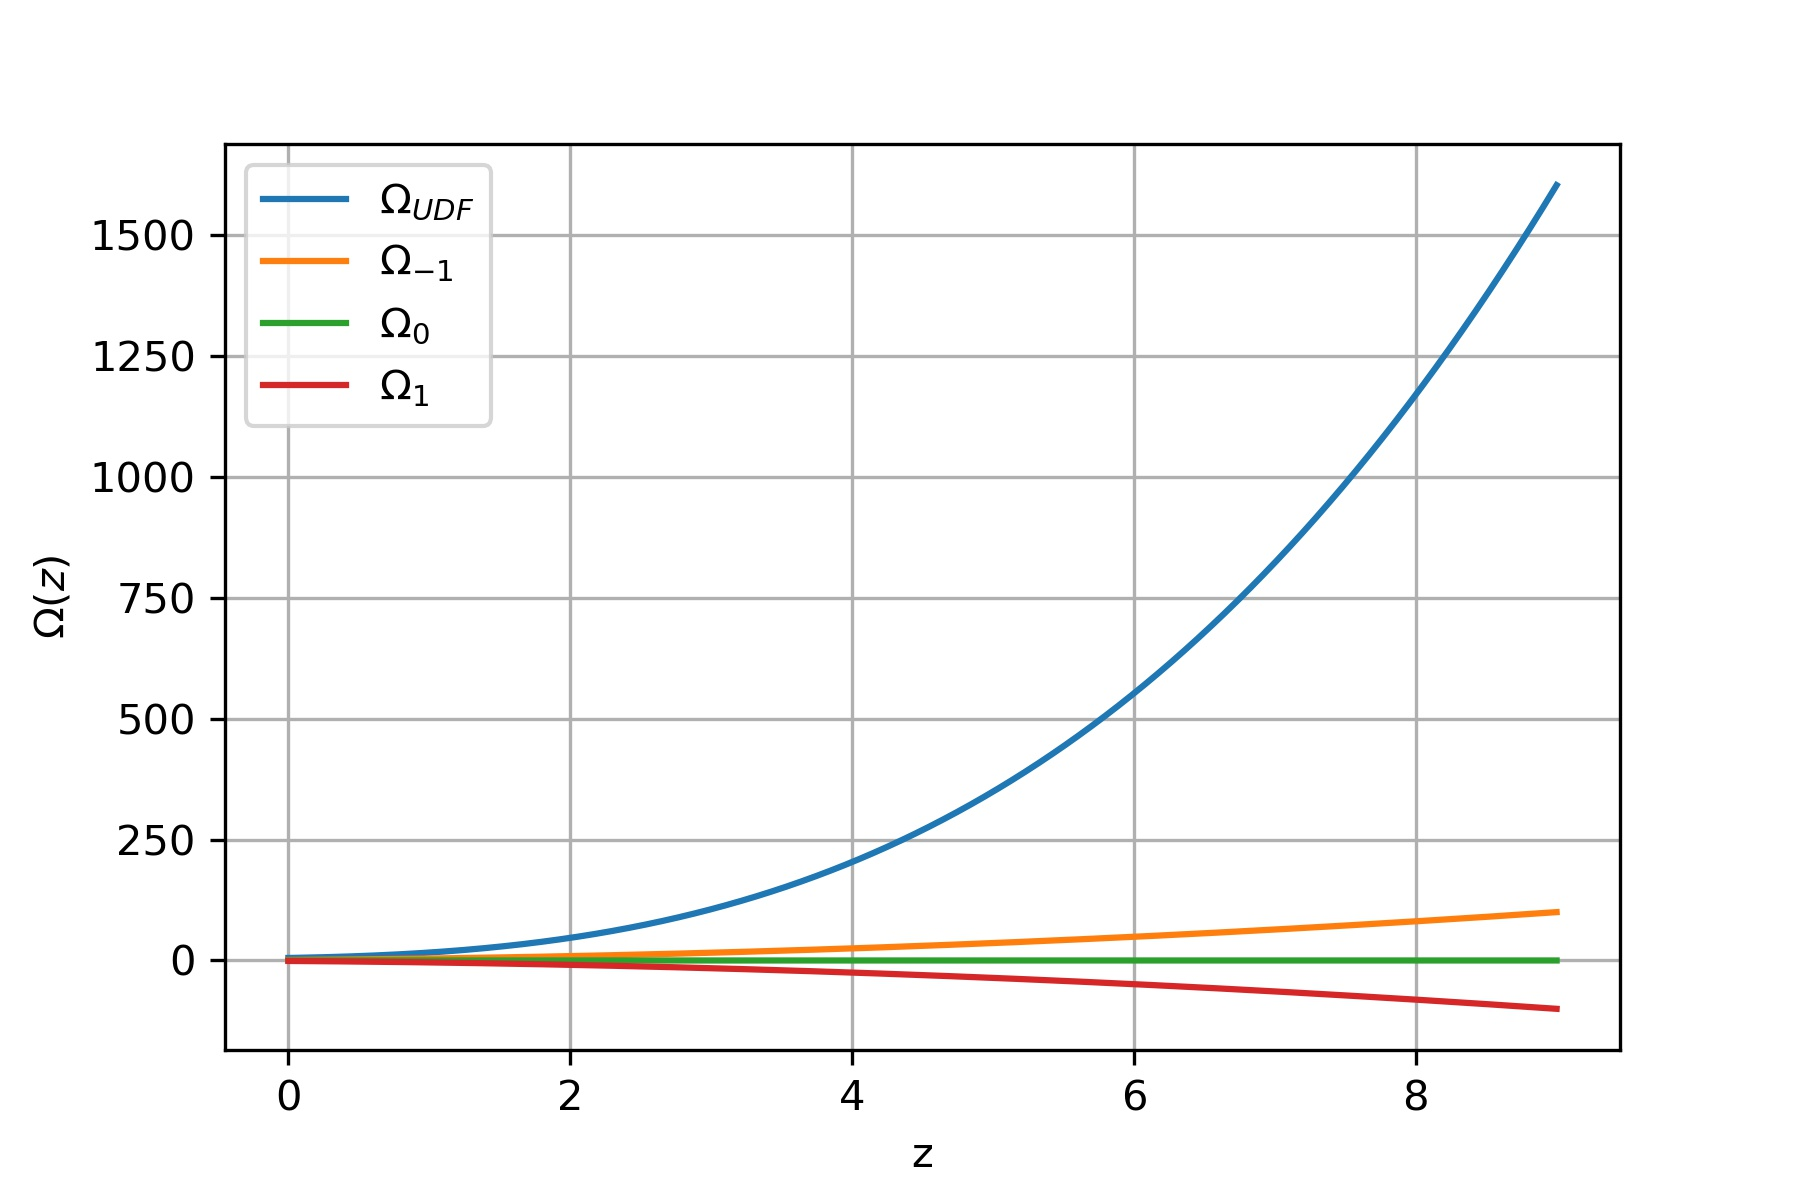
\includegraphics[width=\textwidth]{./Images/UDF_Om.jpg}
		%\caption{Taking the various parameters as in the previous cases, the figure shows 			the fractional energy density of the Chaplygin gas fluid as well as for the 				different curvature cases.It is important to point out here that the fractional 			energy density of the different curvatures are non-linear, but increases much 				slower than the Chaplygin gas fractional energy density for the chosen parameters.}
		\label{fig:UDFFracEnDen}
    \end{minipage}
\end{figure}

\end{frame}

\subsection{Acceleration of a for PPUDF case}
\begin{frame}
\frametitle{\insertsectionhead}
\framesubtitle{\insertsubsectionhead}
\fontsize{8pt}{7.2}\selectfont
\begin{itemize}
\item Acceleration of a:
\fontsize{6pt}{7.2}\selectfont
\begin{equation}\label{eq:RayUDF}
\begin{split}
\frac{\ddot{a}}{a} &= -\frac{A}{2}\bracc{2P_{a}-\frac{3}{2}P_{b}\brac{\frac{3}{2}a+a^{-1}}+Ca^{-3}}.\\
\end{split}
\end{equation}
\fontsize{8pt}{7.2}\selectfont
\item Deceleration parameter $q\equiv-\frac{\ddot{a}a}{\dot{a}^{2}}$
\fontsize{6pt}{7.2}\selectfont
\begin{equation}\label{eq:UDFq}
\begin{split}
q &= \frac{A\bracc{2P_{a}-\frac{3}{2}P_{b}\brac{\frac{3}{2}\brac{1+z}^{-1}+\brac{1+z}}+C\brac{1+z}^{3}}}{2A\brac{-P_{a}+\frac{3}{4}P_{b}\bracc{\brac{1+z}^{-1}-2\brac{1+z}}+C\brac{1+z}^{3}} -\kappa F \brac{1+z}^{2}}.        \\
\end{split}
\end{equation}
\end{itemize}

\begin{figure}[ht]
    \begin{minipage}{0.49\linewidth}
        \centering
        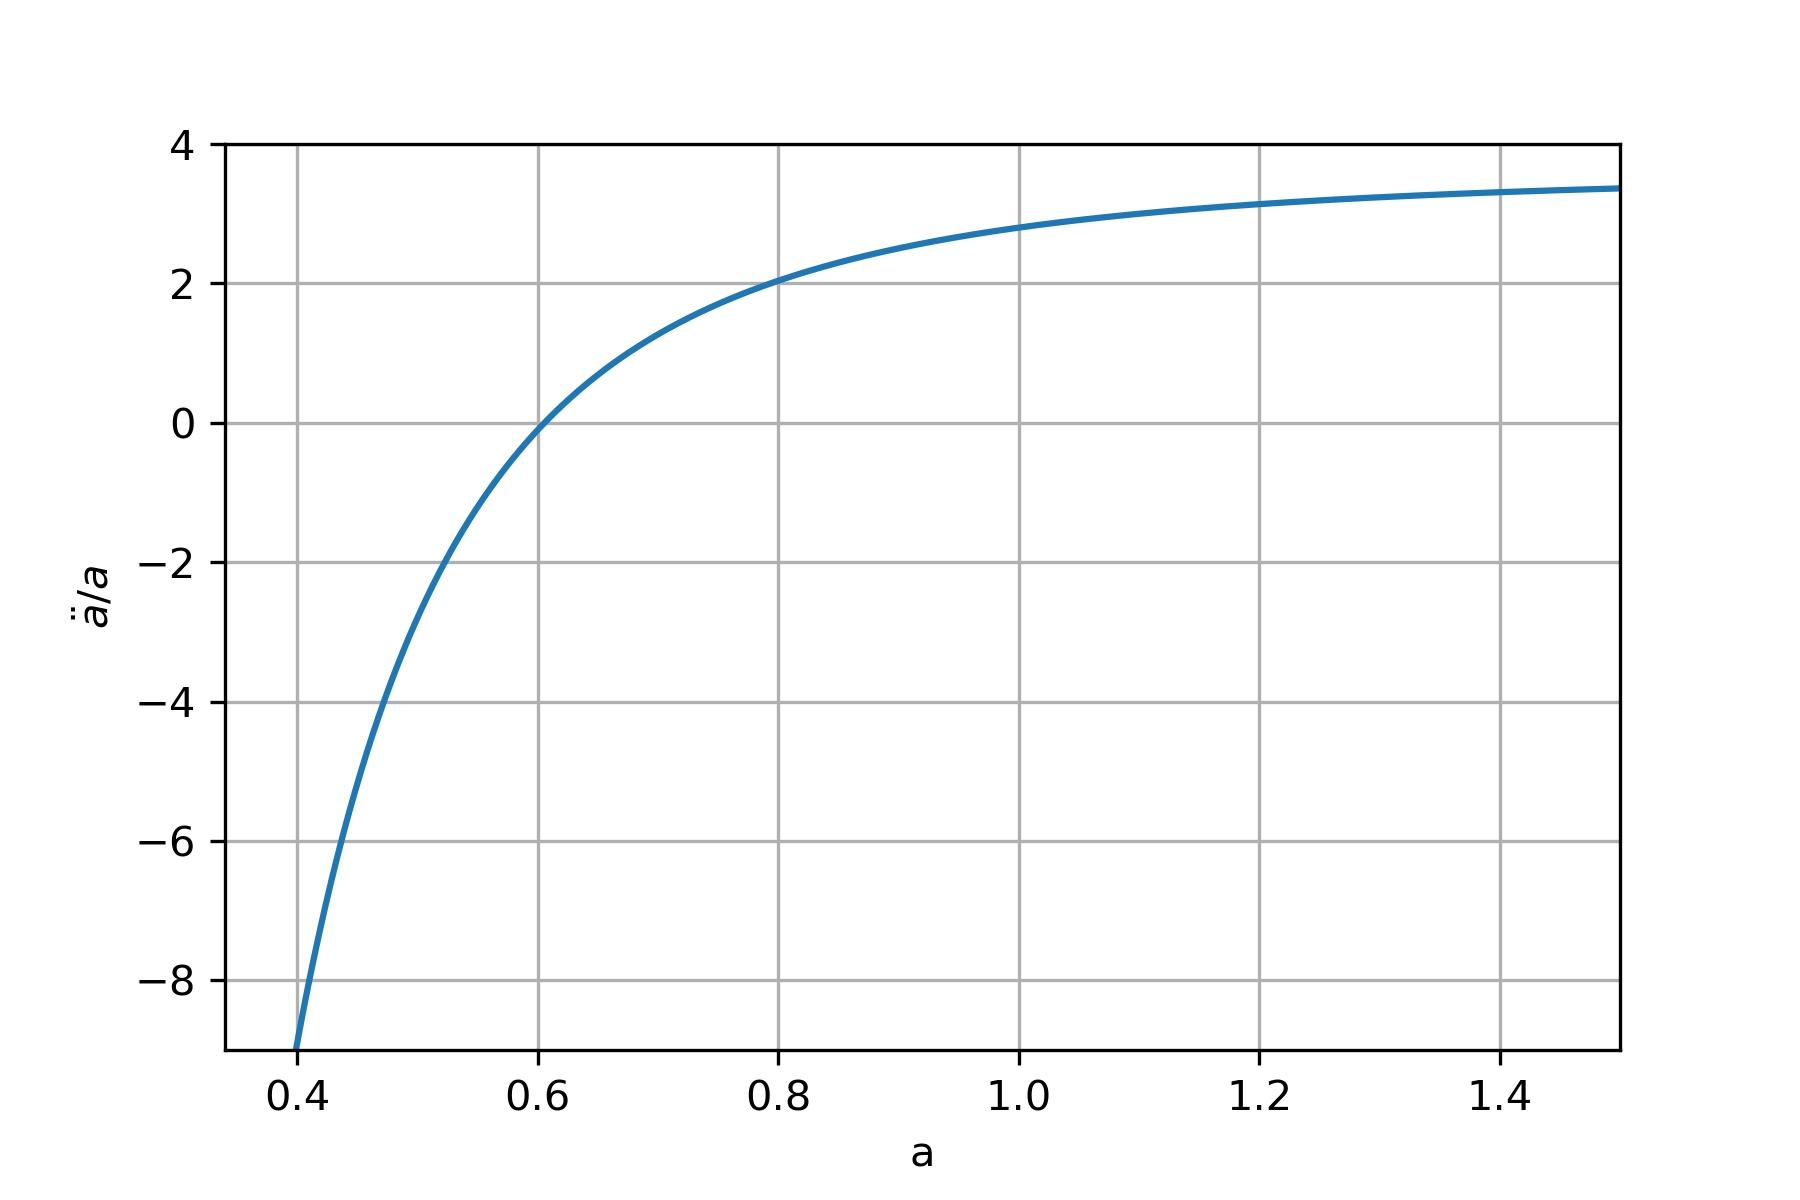
\includegraphics[width=\textwidth]{./Images/UDF_addot.jpg}
		\label{fig:ch_ddot}
    \end{minipage}
    \begin{minipage}{0.49\linewidth}
        \centering
        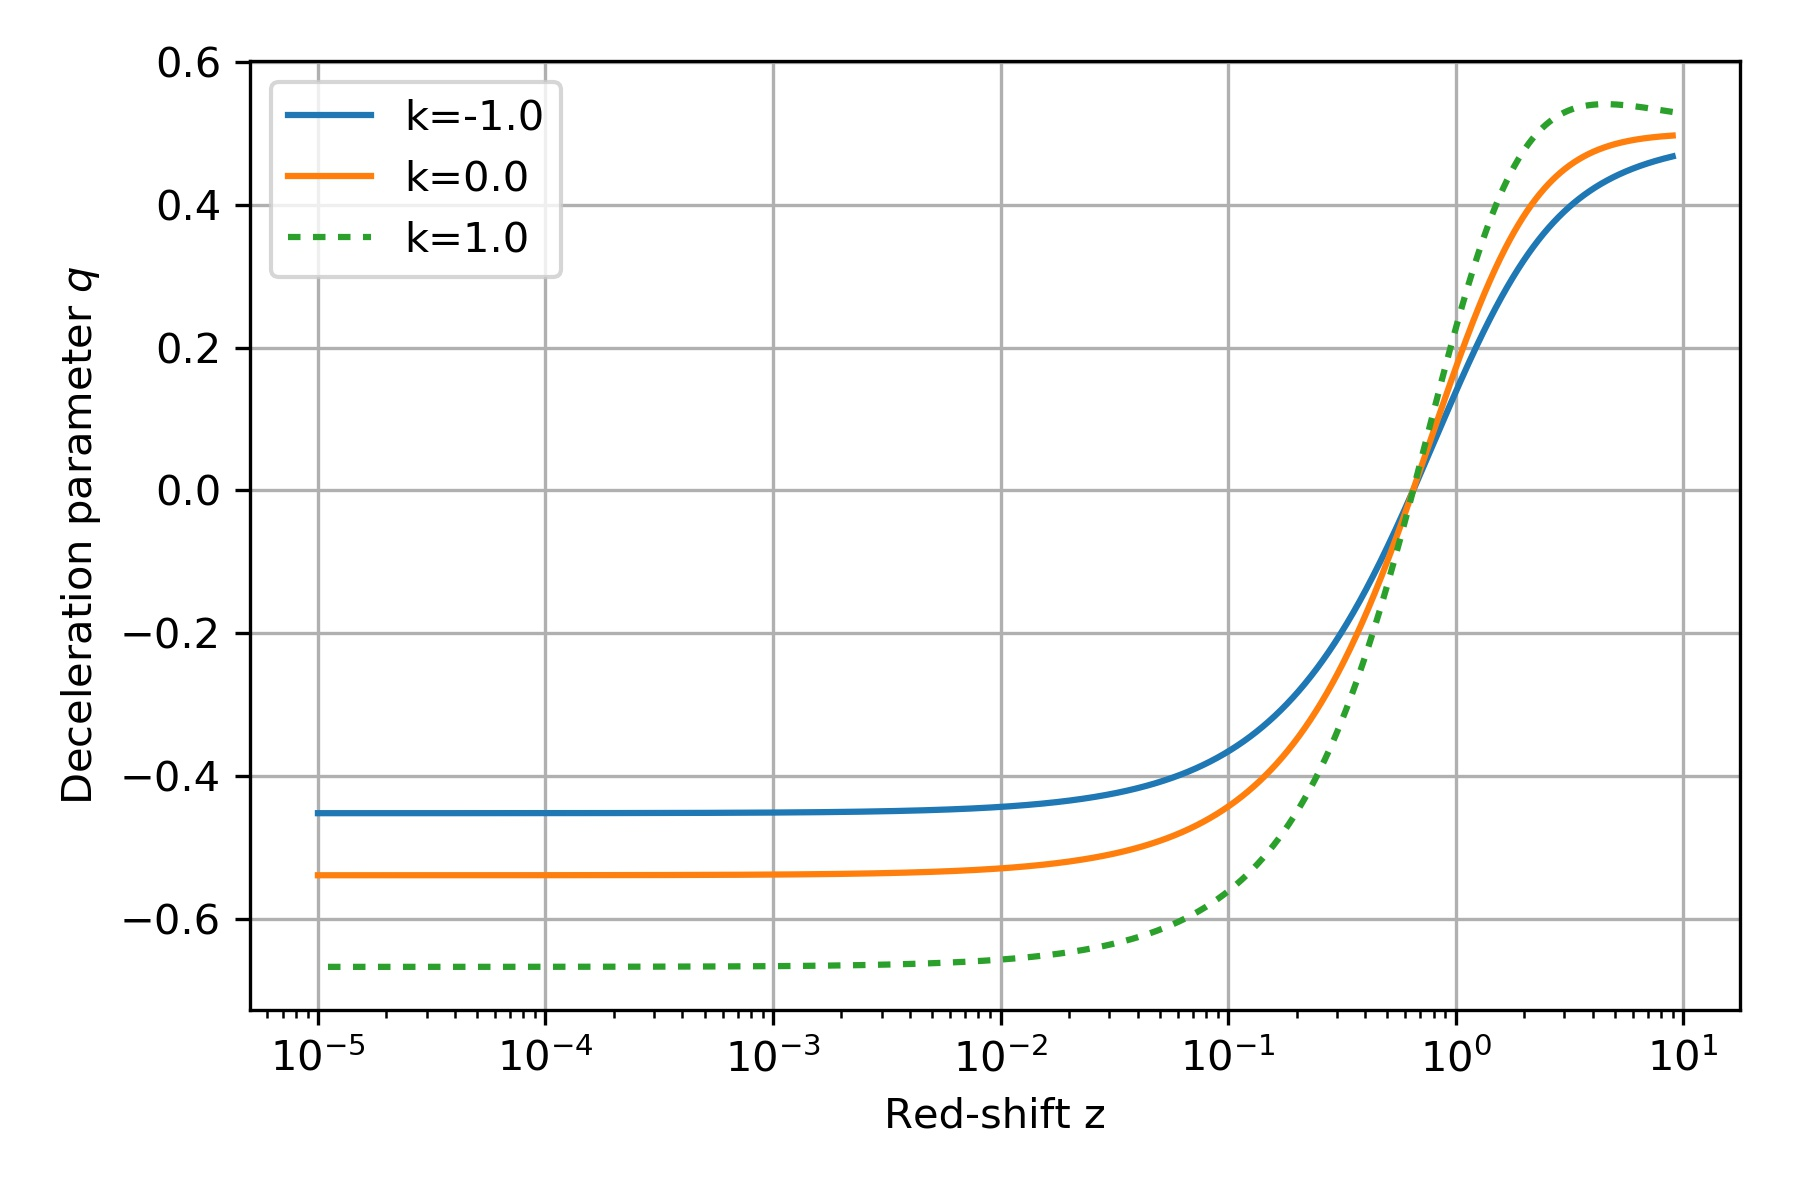
\includegraphics[width=\textwidth]{./Images/UDF_q.jpg}
		\label{fig:Chq}
    \end{minipage}
\end{figure}
\end{frame}

\section{Conclusions}
\begin{frame}
\begin{itemize}
\frametitle{\insertsectionhead}

\item stuff
\end{itemize}
\end{frame}


\begin{frame}
\bibliographystyle{unsrt}                               
\bibliography{./References/References} 
\end{frame}
}


\end{document}